\documentclass{article}

\usepackage{fullpage}
\usepackage[latin1]{inputenc}
\usepackage[danish]{babel}
\usepackage{listings}
\usepackage{caption}
\usepackage[table]{xcolor}
\usepackage{amssymb}
\usepackage{amsmath}
\usepackage{fancyhdr}
\usepackage{lastpage}
\usepackage{parskip}
\usepackage{abstract}
\usepackage{url}
\usepackage{float}
\usepackage{enumitem}
\usepackage[all]{xy}
\usepackage{amstext}
\usepackage{fancybox}
\usepackage{amsmath}
\usepackage{graphicx}
\usepackage{subfigure}
\usepackage[bottom]{footmisc}
\usepackage{hyperref}
\usepackage{tikz}
\usepackage{makecell}

% bootstrap label style highlighting
\newcommand\hw[2][]{\tikz[overlay]\node[fill=blue!20,inner sep=1pt, anchor=text, rectangle, rounded corners=0.1mm,#1] {#2};\phantom{#2}}

% styling
\newcommand{\code}[1]{\texttt{#1}}

% diagrams
\newcommand{\switch}[1]%
  {\ovalbox{\text{\begin{minipage}{1.2in}\centering #1\end{minipage}}}}
\newcommand{\minibox}[1]%
  {\ovalbox{\text{\begin{minipage}{0.85in}\centering #1\end{minipage}}}}

\pagestyle{fancy}
\fancyhf{}
\setlength{\parindent}{0pt}
\setlength{\headheight}{15pt}
\setlength{\headsep}{25pt}
\lfoot{Side \thepage{} af \pageref{LastPage}}
\rfoot{09/12-2013}
\lhead{Embedded Systems}
\chead{Assignment 3}
\rhead{}

\title{Assignment 3}
\date{09.12.2013}
\author{
  Simon Altschuler\\
  \code{s123563}
  \and
  Markus F�revaag\\
  \code{s123692}
}

\begin{document}
\maketitle
\centerline{Gruppens arbejde har v�ret fordelt lige i forbindelse med udarbejdelse
af opgaven og rapporten.}
\clearpage

\tableofcontents
\clearpage

\section{Introduktion} % Norsk
Vi har i denne oppgave integrert vaares MWI filter fra A2 om til en
co-processor som styres av processoren i vaares tidligere system. De
kommunsirer overbussen og er ikke direkte forbundet.

Dette gjoer at vi kan oppnaa en helt annen ydelse naar det gjelder
analysen av dataen, resulterende en endnu mer realistisk loesning av et
komplett inlejret system.

\section{Problemstilling}
\subsection{Fokus}
Skal v�lge at fokuserer p� st�rrelse/power/hastighed

\subsection{Algorithm}
Skal ud fra fokus v�lge en passende algoritme

\section{Design}
\subsection{Fokus}
Vi v�lger at fokuserer p� hastighed, st�rrelse er
irrelevant. Energiforbrug er af mindre betydning, men er stadig v�rd
at overveje. En sk�rm vil alligevel v�re den klart mest energim�ssigt
kr�vende enhed.

At bruge 30 registre vs at bruge 4 og loade tilbage. Vi bruger 30+lidt
for at undg� ekstra load.


\section{Implementation}
\subsection{Overordnet}
\begin{figure}[H]
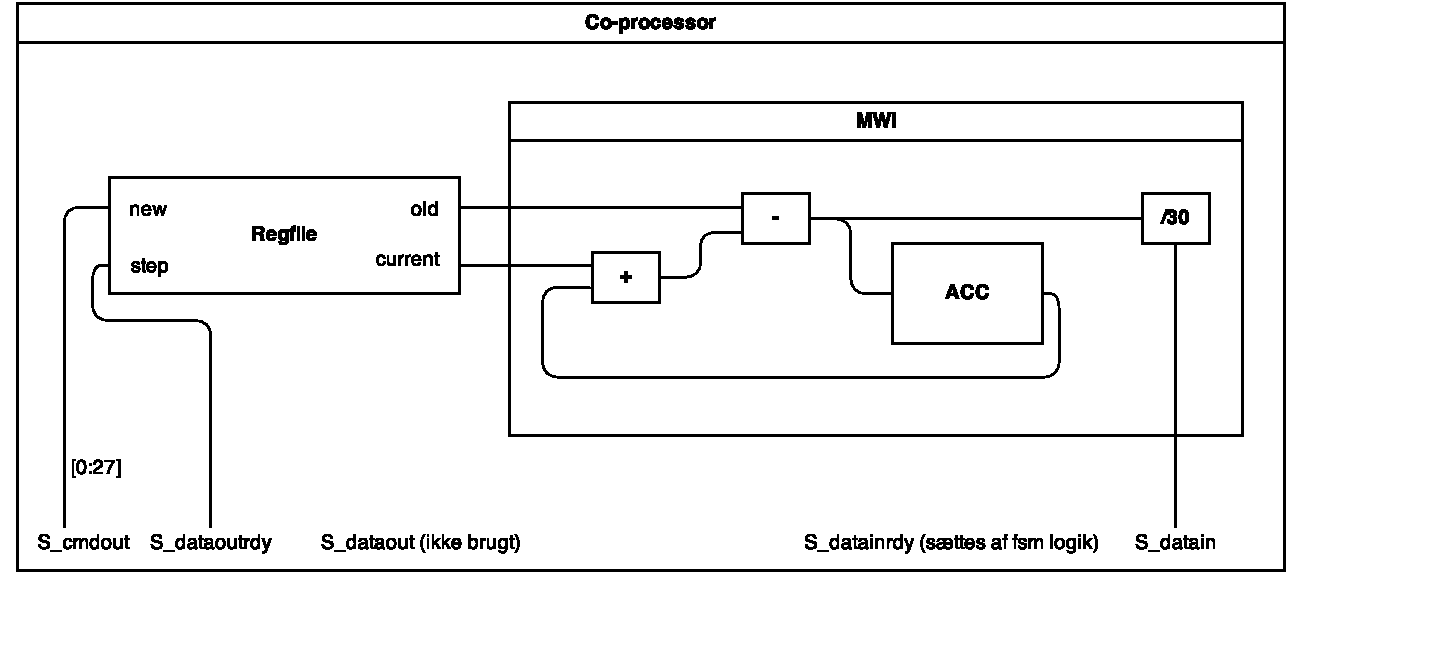
\includegraphics[width=18cm]{diagrams/copro.pdf}
\label{fig:schematic}
\caption{Skema over MWI co-processor implementationen}
\end{figure}

Bruger positive v�rdier da vi ved det er fucking fedt. Le fak?

\subsection{Register komponent}
Bruger 30 registre
Beskriv ``pointer'' metoden
Beh�ver ikke at tjekke hvor mange samples der er observeret fordi registre som standard = 0

\subsection{MWI udregning}

\section{Test}
Tester alle komponenter individuelt
Sv�rt at teste bus integration automatisk


\section{Resultater}
Antal cycles i forhold til uden copro


\section{Konlusion}

\section{K�rsel}

\end{document}
